% Tutto quello riguardante il progetto andrà in questo capitolo

\chapter{Il progetto}\label{chap:project}
\note{Aiuto i tempi verbaliii! Al futuro? Passato? mi metto in prima persona?}
\section{Presentazione progetto}
Il progetto proposto dall'azienda per il lavoro di stage consisteva nella progettazione e nello sviluppo di un prototipo di applicazione chat per dispositivi mobili. Le funzionalità che il prodotto presenta sono allineate alle soluzioni già implementate in ambiente web, invece per quanto riguarda la parte grafica, doveva rispettare lo stile dell'omonimo modulo Teamwork, in fase di riprogettazione. Tale prodotto è stato sviluppato utilizzando il framework React Native, ed è stato reso disponibile sia per sistemi Android che iOS.

\section{Interesse aziendale}
L'applicazione Teamwork sviluppata si appoggerà al software OpenChat\footnote{\url{https://github.com/ZeXtras/OpenChat}}, modulo open source sviluppato da Zextras disponibile come Zimlet su Zimbra, che richiede l'installazione di Zextras core.
L'obbiettivo dell'azienda era di ottenere al termine dello stage un prototipo con almeno le funzionalità base di OpenChat su mobile, in modo tale da:
\begin{itemize}
	\item verificare l'effettiva utilità del progetto;
	\item studiare le migliori soluzioni progettuali per un'ambito \unsure{ancora inesplorato} dall'azienda poiché differente da quello dei prodotti già sviluppati;
	\item validare le tecnologie utilizzate e, eventualmente, proporre nuovi framework di sviluppo;
	\item ampliare e/o modificare le proprie UX guidelines in base alle differenze tra dispositivi mobile e desktop.
\end{itemize}


\section{Piano di lavoro}
Il progetto di stage proposto dall'azienda è stato sviluppato da due stagisti e prevedeva un lavoro di 320 ore ciascuno, così suddivide:
\begin{itemize}
	\item Formazione (40h): introduzione a Zimbra, Zextras, agli strumenti e alle procedure aziendali; un consulente esterno, inoltre, ha provveduto alla formazione sulle tecnologie da utilizzare per il progetto, quali React Native ed Expo, con le quali anche l'azienda ospitante si interfaccia per la prima volta;
	\item  Progettazione UX (40h): studio e realizzazione di alcuni wireframe dell'app prendendo spunto dall’attuale sistema di chat sviluppato per il web;
	\item Progettazione architetturale (40h): progettazione dell’architettura client/server necessaria per l’implementazione dell'applicazione seguendo le bozze dell’UX;
	\item Implementazione (200h): sviluppo dell’applicazione con lo scopo di raggiungere un prototipo funzionante.
	
\end{itemize}

\section{Pianificazione di progetto}
Successivamente al periodo di formazione è stato pianificato in maggior dettaglio il lavoro da svolgere. Le otto settimane di stage sono state suddivise in quattro sprint di due settimane ognuno, riuscendo così a sincronizzare lo sviluppo dell'applicazione con gli sprint degli altri progetti seguiti dall'azienda. \\ Al fine di \mmh{simulare}{metterei anche seguire} il metodo lavorativo aziendale, è stata associata una versione di release del prototipo per ognuno dei quattro sprint decisi. \postit{le loro sono vere release le nostre no ovviamente! Non ci darei peso sinceramente} \\
I quattro sprint sono stati così suddivisi:
\begin{figure}[H] 
	\centering
	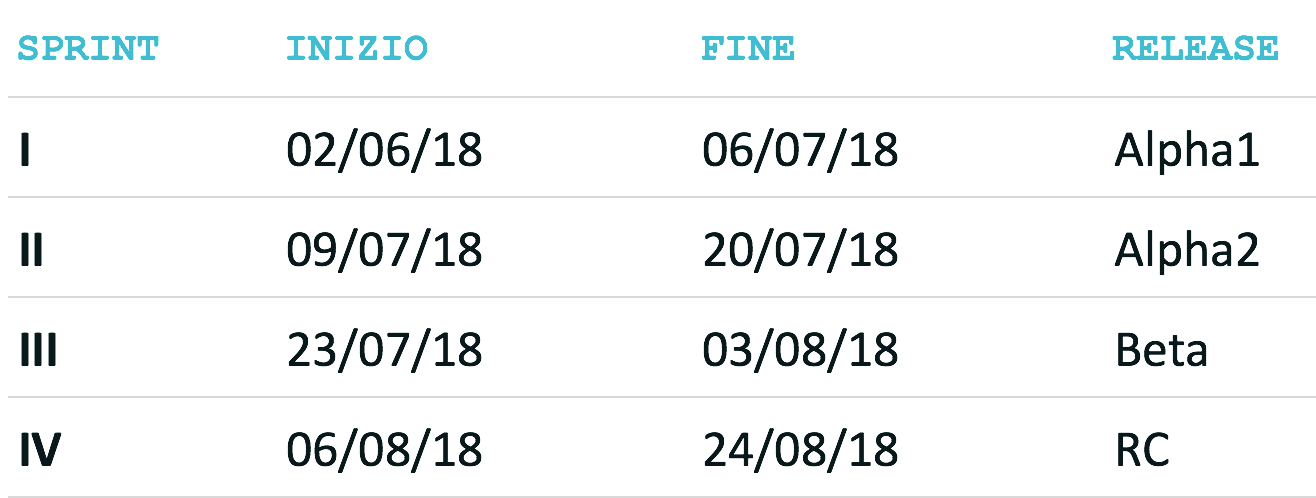
\includegraphics[scale=0.5]{sprint}
	\caption{Definizione sprint}
	\label{fig:sprint}
\end{figure}

\note{mmm fare una tabella decente}


\newcolumntype{C}[1]{>{\centering\arraybackslash}p{#1}}
\note{Possibile tabella}
\begin{table}[H]
\centering
\begin{tabular}{C{2.8cm} C{2.8cm} C{2.8cm} C{2.8cm}}
\hline
\textbf{Sprint} & \textbf{Inizio} & \textbf{Fine} & \textbf{Release} \\ \hline
I               & 02/06/18        & 06/07/18      & Alpha1           \\
II              & 09/07/18        & 20/07/18      & Alpha2           \\
III             & 23/07/18        & 03/08/18      & Beta             \\
IV              & 06/08/18        & 24/08/18      & RC               \\ \hline
\end{tabular}
\end{table}

\subsection{Gli Sprint}
\note{Fare una tabella BELLISSIMA in excel con il riassunto}
Sprint: Alpha 1
\begin{itemize}
	\item Setup progetto (8)
	\begin{itemize}
		\item Expo
		\item TyperScript	
		\item Repo git + submodule OpenChat
		\item Docker + immagine Zimbra\_8.8.8 + ZeXtras
	\end{itemize}
	\item Login
	\item Register session
	\item Strategy
\end{itemize}

\subsection{II Sprint}
\note{Fare una tabella BELLISSIMA in excel con il riassunto}
\subsection{III Sprint}
\note{Fare una tabella BELLISSIMA in excel con il riassunto}
\subsection{IV Sprint}
\note{Fare una tabella BELLISSIMA in excel con il riassunto}
